% !TeX root = surprises.tex

\selectlanguage{hebrew}

\chapter{משפטים מגיאומטריה וטריגונומטרה}\label{a.trig}

%%%%%%%%%%%%%%%%%%%%%%%%%%%%%%%%%%%%%%%%%%%%%%%%%%%%%%%%%%%%%%%

נספח זה מביא משפטים מגיאומטריה וטריגונומטרה שייתכן שהם לא מוכרים לקורא וכן משפטים מוכרים שהוכחותיהם לא מוכרות. סעיף%
~\ref{a.triangles}
מציג שלוש נוסחאות לחישוב השטח של משולש. סעיף%
~\ref{a.trig-identities}
מוכיח זהיות טריגונומטריות. למרות שהנוסחאות והשוויונות מוכרות ברובן, לעתים תלמידים זוכרים אותן בעל-פה או מחפשים אותן בספרים בלי שאי-פעם ראו את ההוכחות. בסעיפים הבאים נמצאות הוכחות של משפטים מתקדמים בגיאומטריה: משפטים על חוצי זוויות (סעיף%
~\ref{a.bisector}),
המשפט של
\L{Ptolemy}
על הקשר בין הצלעות והאלכסונים של מרובע חסום במעגל (סעיף%
~\ref{a.ptolemy}),
המשפט של
\L{Ceva}
על הקשר בין שלושה קטעי קו של משולש (סעיף%
~\ref{a.ceva}),
והמשפט של
\L{Menelaus}
על קטעי הקו של חותך מעגל (סעיף%
~\ref{a.menelaus}).

%%%%%%%%%%%%%%%%%%%%%%%%%%%%%%%%%%%%%%%%%%%%%%%%%%%%%%%%%%%

\section{משפטים על משולשים}\label{a.triangles}


%%%%%%%%%%%%%%%%%%%%%%%%%%%%%%%%%%%%%%%%%%%%%%%%%%%%%%%%%%%

\subsection{חישוב השטח של משולש}
\index{Triangle!computing the area|(}

הנוסחה הסנדרטית לחישוב השטח של משולש מהבסיס והגובה ידועה היטב. ניתן להוכיח אותה בדרכים גיאומטרייות שונות.

\begin{theorem} 
השטח של משולש 
$\triangle ABC$
ניתן על ידי:
\begin{equation}\label{eq.area-from-base}
\triangle ABC=\frac{1}{2}bh\,,
\end{equation}
כאשר הבסיס 
$b$
הוא אחד מצלעות המשולש ו-%
$h$
הוא הגובה ל-%
$b$
מהקודקוד הנגדי
(איור~%
\ref{f.area-base-height-1}).
\end{theorem}

\begin{proof}
איור~%
\ref{f.area-base-height-2}
מראה שעל ידי "חיתוך" המשולש במחצית גובהו, נוכל "להזיז" את המשולשים הצבועים כדי לבנות מלבן ששטחו שווה לשטח המשולש. בסיס המלבן הוא 
$b$
וגובהו
$h/2$.
\end{proof}

\begin{figure}[t]
\centering
\selectlanguage{hebrew}
\subcaptionbox{%
חישוב שטח משולש מהבסיס והגובה
\label{f.area-base-height-1}}
[.45\textwidth]
{
\centering
\begin{tikzpicture}[scale=.7]
\coordinate (A) at (0,0);
\coordinate (C) at (7,0);
\path[name path=ab] (A) -- +(60:5.5);
\path[name path=cb] (C) -- +(140:7);
\path[name intersections={of=ab and cb,by={B}}];
\draw (A) -- node[below] {$b$} (C) -- node[above] {$a$} (B) -- node[above,xshift=-2pt] {$c$}  cycle;
\node[left] at (A) {$A$};
\node[above right,xshift=4pt] at (A) {$\theta$};
\node[above] at (B) {$B$};
\node[right] at (C) {$C$};
\draw (B) -- node[right,xshift=-1pt,yshift=-12pt] {$h=c\sin\theta$} 
  (B|-A) coordinate (H);
\draw[rotate=90] (H) rectangle +(8pt,8pt);
\end{tikzpicture}
}
\hspace{3em}
\subcaptionbox{%
חישוב שטח משולש מהבסיס והגובה
\label{f.area-base-height-2}}
[.45\textwidth]
{
\centering
\begin{tikzpicture}[scale=.7]
\coordinate (A) at (0,0);
\coordinate (C) at (7,0);
\path[name path=ab] (A) -- +(60:5.5);
\path[name path=cb] (C) -- +(140:7);
\path[name intersections={of=ab and cb,by={B}}];
\node[left] at (A) {$A$};
\node[above] at (B) {$B$};
\node[right] at (C) {$C$};
\path (B) -- node[right,near end] {$h/2$} (B|-A) coordinate (H);
\draw[rotate=90] (H) rectangle +(8pt,8pt);
\coordinate (K) at ($(H)!.5!(B)$);
\draw (A) -- node[below] {$b$} (C);
\draw (H) -- (K);
\coordinate (KA) at (K -| A);
\coordinate (KAB) at ($(A)!.5!(B)$);
\fill[color=white!50!red] (A) -- (KA) -- (KAB) -- cycle;
\fill[color=white!50!red] (B) -- (KAB) -- (K) -- cycle;
\coordinate (KC) at (K -| C);
\coordinate (KBC) at ($(B)!.5!(C)$);
\fill[color=white!50!blue] (C) -- (KC) -- (KBC) -- cycle;
\fill[color=white!50!blue] (B) -- (KBC) -- (K) -- cycle;
\draw[very thick,dashed] (A) -- (K -| A) -- (K -| C) -- (C);
\draw[very thick,dashed] (A) -- (B) -- (K);
\draw[very thick,dashed] (B) -- (C);
\path (K) -- node[inner sep=1pt, fill=white,right,
                 xshift=2pt,yshift=-7pt] {$h/2$} (B);
\end{tikzpicture}
}
\end{figure}

\begin{theorem}
השטח של משולש 
$\triangle ABC$
ניתן על ידי:
\begin{equation}\label{eq.area-from-sine}
\triangle ABC = \frac{1}{2}bc\sin \theta\,.
\end{equation}
\end{theorem}
\begin{proof}
ממשפט%
~\ref{eq.area-from-base}
כאשר
$h=c\sin \theta$.
\end{proof}

%%%%%%%%%%%%%%%%%%%%%%%%%%%%%%%%%%%%%%%%%%%%%%%%%%%%%%%%%%%

\index{Triangle!Heron's formula}
\begin{theorem}[Heron]\label{thm.heron}
השטח של משולש 
$\triangle ABC$
ניתן על ידי:
\[
\triangle ABC = \sqrt{s(s-a)(s-b)(s-c)}\,,
\]
כאשר 
$s$,
מחצית ההיקף של המשולש, שווה ל-%
$\frac{1}{2}(a+b+c)$.
\end{theorem}

\begin{proof}
רדיוס של מעגל ומשיק החותך את רדיוס ניצבים אחד לשני. בנוסף, האורכים של קטעי הקו של שני משיקים מאותה נקודה למעגל שווים. לכן
(איור%
~\ref{f.inscribed-trig}):%
\footnote{%
זה מראה שה-%
\L{incenter}%
\index{Triangle!incenter}\index{Triangle!inscribed circle}
מרכז המעגל החסום הוא נקודת החיתןך המשותפת לשלושת חוצי הזווית.}
\[
\triangle AOB'\cong \triangle AOC',\quad
\triangle BOA'\cong\triangle BOC',\quad
\triangle COA'\cong \triangle COB'\,.
\]
\begin{figure}[bt]
\begin{center}
\begin{tikzpicture}[scale=1.8]
% Draw base and path two lines at known angles
\draw (0,0) coordinate (a) node[xshift=-6pt] {$A$} -- (0:6) coordinate (b) node[xshift=6pt] {$B$};
\path[name path=ac] (a) -- +(50:4);
\path[name path=bc] (b) -- +(150:5);
% Get their intersection and draw lines between vertices
\path[name intersections={of=ac and bc,by=c}];
\node[above] at (c) {$C$};
\draw (a) -- (c) -- (b) -- (a);
% Label angles with tick marks
\draw (a) ++(0:4mm) arc (0:50:4mm);
\draw (a) ++(10:3.5mm) -- +(10:1mm);
\draw (a) ++(15:3.5mm) -- +(15:1mm);
\draw (a) ++(35:3.5mm) -- +(35:1mm);
\draw (a) ++(40:3.5mm) -- +(45:1mm);
\draw (b) ++(150:5mm) arc (150:180:5mm);
\draw (b) ++(157.5:4.5mm) -- +(157.5:1mm);
\draw (b) ++(172.5:4.5mm) -- +(172.5:1mm);
\draw (c) ++(230:3mm) arc (230:330:3mm);
\draw (c) ++(250:2.4mm) -- +(250:.9mm);
\draw (c) ++(255:2.4mm) -- +(255:.9mm);
\draw (c) ++(260:2.4mm) -- +(260:.9mm);
\draw (c) ++(300:2.4mm) -- +(300:.9mm);
\draw (c) ++(305:2.4mm) -- +(305:.9mm);
\draw (c) ++(310:2.4mm) -- +(310:.9mm);
% Path bisectors of two lines
\path[name path=bia] (a) -- +(25:3.5);
\path[name path=bib] (b) -- +(165:5);
% Intersection of angle bisectors
\path [name intersections={of=bia and bib,by=center}];
% Draw angle bisectors to center
\draw (a) -- (center);
\draw (c) -- (center);
\draw (b) -- (center);
% Draw radii
\draw (center) -- node[left] {$r$} ($(a)!(center)!(b)$) node[below,yshift=-2pt] {$C'$} coordinate (ap);
\draw (center) -- node[left,yshift=-4pt] {$r$} ($(a)!(center)!(c)$) node[above left] {$B'$} coordinate (bp);
\draw (center) -- node[right] {$r$} ($(b)!(center)!(c)$) node[above right] {$A'$} coordinate (cp);
% Draw dots
\vertex{center};
\node[above,xshift=3pt,yshift=7pt] at (center) {$O$};
% Draw right angle squares
\draw (ap) -- ++(90:4pt) -- ++(0:4pt) -- ++(-90:4pt);
\draw (bp) -- ++(-40:4pt) -- ++(-130:4pt) -- ++(-220:4pt);
\draw (cp) -- ++(-30:4pt) -- ++(-120:4pt) -- ++(-210:4pt);
% Labels of angles
\node[above,xshift=5pt,yshift=18pt] at (center) {$\gamma/2$};
\node[above left,xshift=-4pt,yshift=18pt] at (center) {$\gamma/2$};
\node[above right,xshift=3pt,yshift=-3pt] at (center) {$\beta/2$};
\node[below right,yshift=-3pt] at (center) {$\beta/2$};
\node[left,xshift=-5pt,yshift=2pt] at (center) {$\alpha/2$};
\node[below left,xshift=2pt,yshift=-4pt] at (center) {$\alpha/2$};
% Labels of line segments (names of points are weird...)
\path (a) -- node[below,yshift=-2pt] {$u$} (ap);
\path (a) -- node[left, xshift=-2pt] {$u$} (bp);
\path (b) -- node[above,yshift=2pt]  {$v$} (cp);
\path (b) -- node[below,xshift=-2pt] {$v$} (ap);
\path (c) -- node[above,xshift=-2pt] {$w$} (bp);
\path (c) -- node[above,xshift=2pt]  {$w$} (cp);
% Labels of sides
\draw[<->] ($(a)+(0,-10pt)$) -- node[fill=white] {$c$} 
           ($(b)+(0,-10pt)$);
\draw[<->] ($(a)+(-10pt,8pt)$) -- node[fill=white] {$b$}
           ($(c)+(-10pt,8pt)$);
\draw[<->] ($(b)+(6pt,10pt)$) -- node[fill=white] {$c$}
           ($(c)+(6pt,10pt)$);
% Inscribed circle
\node[very thick,dotted,draw,circle through=(ap)] at (center) {};
\end{tikzpicture}
\end{center}
\caption{משולש החוסם מעגל}\label{f.inscribed-trig}
\end{figure}

\newpage

השטח של
$\triangle ABC$
הוא סכום השטחים של ששת המשולשים הללו. הגובה של כל  אחד מהמשולשים הוא 
$r$,
הרדיוס של המעגל החסום, ולכן:
\begin{eqnlabels}
\triangle ABC&=&\triangle AOB'\!+\!\triangle AOC'\!+\!\triangle BOA'\!+\!\triangle BOC'\!+\!\triangle COA'\!+\!\triangle COB'\\
\triangle ABC&=&\frac{1}{2}r(u+u+v+v+w+w)\\
\triangle ABC&=&\frac{1}{2}r(a+b+c)\\
\triangle ABC&=&rs \label{eq.area-heron}\,.
\end{eqnlabels}
נגדיר עכשיו את הצלעות מהטנגסים של הזוויות המרכזיות:
\begin{displaymath}
\tan \frac{\alpha}{2} = \frac{u}{r},\quad
\tan \frac{\beta}{2} = \frac{v}{r},\quad
\tan \frac{\gamma}{2} = \frac{w}{r}\,.
\end{displaymath}
מההגדרות הללו ומ-%
$s=\frac{1}{2}(2u+2u+2w)$
נקבל:
\[
s = u+v+w = r\left(\tan \frac{\alpha}{2}+\tan \frac{\beta}{2}+\tan \frac{\gamma}{2}\right)\,.
\]
מ-%
$\frac{\alpha}{2}+\frac{\alpha}{2}+\frac{\beta}{2}+\frac{\beta}{2}+\frac{\gamma}{2}+\frac{\gamma}{2}=360^\circ$
נקבל
$\frac{\alpha}{2}+\frac{\beta}{2}+\frac{\gamma}{2}=180^\circ$,
ולפי משפט%
~\ref{thm.tangent3}:
\begin{eqn}
s&=&r\left(\tan \frac{\alpha}{2}\tan \frac{\beta}{2}\tan \frac{\gamma}{2}\right)\\
&=&r\left(\frac{u}{r}\frac{v}{r}\frac{w}{r}\right)=\frac{1}{r^2}(u\,v\,w)\\
r&=&\sqrt{\displaystyle\frac{u\,v\,w}{s}}\,.
\end{eqn}
מנוסחה%
~\ref{eq.area-heron}:
\[
\triangle ABC=rs=s\sqrt{\displaystyle\frac{u\,v\,w}{s}}=\sqrt{s\,u\,v\,w}\,.
\]
הנוסחה של 
\L{Heron}
מתקבלת מ-%
$u=s-a, v=s-b, w=s-c$.
\end{proof}
\index{Triangle!computing the area|)}

%%%%%%%%%%%%%%%%%%%%%%%%%%%%%%%%%%%%%%%%%%%

\section{זהויות טריגונומטריות}\label{a.trig-identities}
\index{Trigonometric identities|(}
\index{Trigonometric identities!sine and cosine of the sum and difference of two angles}

%%%%%%%%%%%%%%%%%%%%%%%%%%%%%%%%%%%%%%%%%%%%%%%%%%%%%%%%%%%

\subsection{הסינוס והקוסינוס של הסכום וההפרש של שתי זוויות} \label{s.sum-of-trig}

\begin{theorem}\label{thm.sum-of-trig}
\begin{eqn}
\sin(\alpha+\beta) &=& \sin\alpha\cos\beta + \cos\alpha\sin\beta\\
\sin(\alpha-\beta) &=& \sin\alpha\cos\beta - \cos\alpha\sin\beta\\
\cos(\alpha+\beta) &=& \cos\alpha\cos\beta - \sin\alpha\sin\beta\\
\cos(\alpha-\beta) &=& \cos\alpha\cos\beta + \sin\alpha\sin\beta\,.
\end{eqn}
\end{theorem}
נוכיח את הנוסחה הראשונה. ניתן לקבל את הנוסחאות האחרות מערכי הסינוס והקוסינוס עבור 
$-\alpha$
ו-%
$90^\circ-\alpha$.
נתון משולש ישר-זווית 
$\triangle ABC$
עם זווית חדה
$\alpha$,
ומשלוש ישר-זווית 
$\triangle ACD$
עם זווית חדה
$\beta$,
ניתן לחברם ולקבל מצולעים עם זווית 
$\alpha+\beta$ (איור.~\ref{f.sin-sum1}).
המצולע השמאלי מופיע לעתים קרובות בהוכחות בספרי לימוד. כאן נביא הוכחות המבוססות על המצולעים במרכז ובימין.
\begin{figure}[tb]
\begin{center}
\begin{tikzpicture}[scale=.85]
\coordinate (A) at (0,0);
\node[below] at (A) {$A$};
\node[right,xshift=6pt,yshift=4pt] at (A) {$\alpha$};
\node[above right,xshift=6pt,yshift=8pt] at (A) {$\beta$};
\coordinate (B) at (3,0);
\node[below] at (B) {$B$};
\path[name path=ac1] (A) -- +(40:4.5);
\path[name path=bc1] (B) -- +(90:3.5);
\path[name intersections={of=ac1 and bc1,by={C}}];
\node[above right] at (C) {$C$};
\draw (A) -- (B) -- (C) -- cycle;
\draw (C) -- ($(C)!2cm!-90:(A)$) coordinate (D) -- (A);
\node[above] at (D) {$D$};
\draw[rotate=90] (B) rectangle +(7pt,7pt);
\draw[rotate=128] (C) rectangle +(7pt,7pt);

\begin{scope}[xshift=4.3cm]
\coordinate (B) at (0,0);
\node[below] at (B) {$B$};
\coordinate (D) at (4,0);
\node[below] at (D) {$D$};
\draw (B) -- +(70:4) coordinate (A);
\node[above] at (A) {$A$};
\draw (A) -- (B) -- (D) -- cycle;

\draw (A) -- (A|-B) coordinate (C);
\node[below] at (C) {$C$};
\node[below left,xshift=2pt,yshift=-18pt] at (A) {$\alpha$};
\node[below right,xshift=0pt,yshift=-14pt] at (A) {$\beta$};
\draw[rotate=90] (C) rectangle +(7pt,7pt);
\draw (C) rectangle +(7pt,7pt);
\end{scope}

\begin{scope}[xshift=9.75cm]
\coordinate (A) at (0,0);
\node[below] at (A) {$A$};
\node[right,xshift=6pt,yshift=5pt] at (A) {$\alpha$};
\node[above right,xshift=4pt,yshift=8pt] at (A) {$\beta$};
\coordinate (B) at (3.5,0);
\node[below] at (B) {$B$};
\draw (A) -- +(70:4.5) coordinate (D);
\node[above] at (D) {$D$};
\path[name path=dc1] (D) -- +(-20:2.5);
\path[name path=bc1] (B) -- +(90:4);
\path[name intersections={of=dc1 and bc1,by={C}}];
\node[above] at (C) {$C$};
\draw[rotate=90] (B) rectangle +(7pt,7pt);
\draw[rotate=-110] (D) rectangle +(7pt,7pt);
\draw (A) -- (B) -- (C) -- (D) -- cycle;
\draw (A) -- (C);
\end{scope}
\end{tikzpicture}
\end{center}
\caption{איורים להכוחת הזהות לסינוס של הסכום של זוויות}\label{f.sin-sum1}
\end{figure}

\begin{proof}(1)
נחשב את השטח של 
$\triangle ABD$
בשתי דרכים שונות: (1) על ידי שימוש בנוסחה%
~\ref{eq.area-from-sine}
על 
$\triangle ABD$,
ו-(2) על ידי שימוש בנוסחה בנפרד על 
$\triangle ABC$
ו-%
$\triangle ADC$ (איור~\ref{f.sin-sum2}).
גם את
$h$
נחשב בשתי דרכים שונות על ידי שימוש בהגדרות של הפונקציות הטריגונומטריות:
\begin{eqn}
\triangle ABD &=& \frac{1}{2}bc\sin(\alpha+\beta)\\
\triangle ABD &=& \triangle ABC+\triangle ADC\\
&=& \frac{1}{2}ch\sin \alpha + \frac{1}{2}bh\sin \beta\\
&=& \frac{1}{2}c(b\cos\beta)\sin \alpha + \frac{1}{2}b(c\cos\alpha)\sin \beta\\
\sin(\alpha+\beta)&=&\sin\alpha\cos\beta+\cos \alpha\sin\beta\,.
\end{eqn}
\end{proof}

\begin{figure}[tb]
\begin{center}
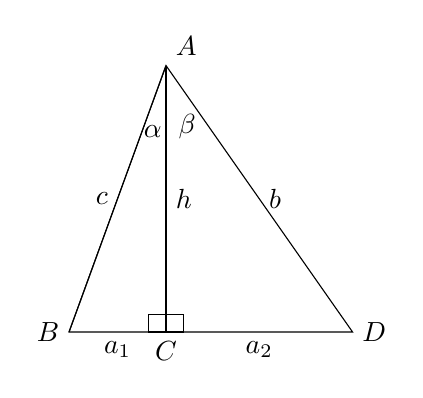
\begin{tikzpicture}[scale=.9]
\coordinate (B) at (0,0);
\node[left] at (B) {$B$};
\coordinate (D) at (4,0);
\node[right] at (D) {$D$};
\draw (B) -- +(70:4) coordinate (A);
\node[above right] at (A) {$A$};
\draw (A) -- node[left] {$c$} (B) -- (D) -- node[right] {$b$} cycle;

\draw (A) -- node[right] {$h$} (A|-B) coordinate (C);
\node[below] at (C) {$C$};
\node[below left,xshift=2pt,yshift=-18pt] at (A) {$\alpha$};
\node[below right,xshift=1pt,yshift=-14pt] at (A) {$\beta$};
\draw[rotate=90] (C) rectangle +(7pt,7pt);
\draw (C) rectangle +(7pt,7pt);
\path (B) -- node[below] {$a_1$} (C) -- node[below] {$a_2$} (D);
\end{tikzpicture}
\end{center}
\caption{חישוב שטח המשולש בשתי דרכים שונות}\label{f.sin-sum2}
\end{figure}
הוכחה השניה משתמשת במשפט שלהלן:
\begin{theorem}
במעגל עם 
\textbf{קוטר}
$1$
אורכו של מיתר התומך בזווית שווה לסינוס של הזווית
(איור.~\ref{f.chord-angle}).
\end{theorem}


\begin{figure}[tb]
\centering
\selectlanguage{hebrew}
\subcaptionbox{כל הזוויות הנתמכות על ידי מיתר שוות
\label{f.chord-angle}}
[.45\textwidth]
{
\centering
\begin{tikzpicture}[scale=.7]

\coordinate (A) at (0,0);
\coordinate (C) at (3,4);
\coordinate (O) at ($(A)!.5!(C)$);
\vertex{O};
\node[left] at (O) {$O$};
\draw (A) -- (C);
\node[draw,circle through=(A),name path=circle] at (O) {};
\coordinate (B) at ($(O)+(10:2.5)$);
\draw (A) -- (B) -- node[left] {$a$} (C);
\draw[rotate=120] (B) rectangle +(8pt,8pt);
\coordinate (D) at ($(O)+(160:2.5)$);
\draw(C) -- (D) -- (B);
\node[above right,xshift=12pt,yshift=12pt] at (A) {$\alpha$};
\node[right,xshift=16pt,yshift=2pt] at (D) {$\alpha$};
\node[below left] at (A) {$A$};
\node[above right] at (C) {$B$};
\node[right] at (B) {$C$};
\node[left] at (D) {$D$};
\end{tikzpicture}
}
\hspace{1em}
\subcaptionbox{מרובע חסום בתוך מעגל
\label{f.trig-quad-circle}}
[.45\textwidth]
{
\centering
\begin{tikzpicture}[scale=.8]
\coordinate (A) at (0,0);
\node[left] at (A) {$A$};
\node[right,xshift=6pt,yshift=5pt] at (A) {$\alpha$};
\node[above right,xshift=4pt,yshift=8pt] at (A) {$\beta$};
\coordinate (B) at (3.5,0);
\node[right] at (B) {$B$};
\draw (A) -- +(70:4.5) coordinate (D);
\node[above left] at (D) {$D$};
\path[name path=dc1] (D) -- +(-20:2.5);
\path[name path=bc1] (B) -- +(90:4);
\path[name intersections={of=dc1 and bc1,by={C}}];
\node[above right] at (C) {$C$};
\draw[rotate=90] (B) rectangle +(9pt,9pt);
\draw[rotate=-110] (D) rectangle +(9pt,9pt);
\draw (A) -- (B) -- (C) -- (D) -- cycle;
\draw (A) -- (C);
\draw (D) -- (B);

\coordinate (O) at ($(A)!.5!(C)$);
\node[draw,circle through=(A),name path=circle] at (O) {};
\node[below right,xshift=6pt,yshift=-4pt] at (D) {$\alpha$};
\node[below,xshift=1pt,yshift=-10pt] at (D) {$\gamma$};
\node[below left,xshift=-6pt,yshift=4pt] at (C) {$\delta$};
\node[below,xshift=-4pt,yshift=-6pt] at (C) {$\gamma$};
\node[above left,xshift=-7pt,yshift=4pt] at (B) {$\delta$};
\node[above,xshift=-4pt,yshift=14pt] at (B) {$\beta$};
\end{tikzpicture}
}
\end{figure}

\begin{proof}
יהי
$\overline{AB}$
קוטר, 
$\angle BAC=\alpha$
ו-%
$D$
כל נקודה אחרת במעגל המייצרת את המשולש
$\triangle BDC$.
בגלל שכל הזוויות שנתמכות על ידי אותו מיתר שוות,
$\angle BDC=\alpha$. 
במשולש ישר-זווית
$\triangle ABC$:
\[
\sin \alpha = \frac{\overline{BC}}{\overline{AB}}=\frac{\overline{BC}}{1}=\overline{BC}\,.
\]
\end{proof}

\begin{proof}(2)
ההוכחה מבוססת על התרשים הימני באיור%
~\ref{f.sin-sum1}
שנמצא גם ב-%
~\ref{f.trig-quad-circle},
כאשר המרובע
$\overline{ABCD}$ 
חסום בתוך מעגל.
\index{Quadrilateral!inscribed in a circle}
לפי משפט
~\ref{thm.quad-circum}
מרובע יכול להיות חסום בתוך מעגל אם ורק אם הסכום שכל זוג של זוויות 
\index{Circumscribed circle} 
נגדיות שווה ל-%
$180^\circ$.
$\angle ADC+\angle ABC=180^\circ$
כי שתי הזוויות הן ישרות. לפי משפט%
~\ref{thm.interior-angles-of-a-polygon}
סכום הזוויות המרכזיות במרובע הוא
$360^\circ$
ולכן
$\angle DAB+\angle DCB=180^\circ$. 



נניח שקוטר המעגל הוא
$1$
(אחרת הכפל הכל באורך הקוטר). הצלעות של המרובע הם:
\[
\overline{BC}=\sin\alpha,\quad \overline{CD}=\sin\beta,\quad \overline{AB}=\sin\gamma,\quad \overline{DA}=\sin\delta\,,
\]
והאלכסונים הם:
\[
\overline{BD}=\sin(\alpha + \beta),\quad \overline{CA}=\sin (\alpha+\gamma)\,.
\]
לפי משפט 
\L{Ptolemy}
\index{Ptolemy's theorem}
(משפט.~\ref{thm.ptolemy})
המכפלה של האלכסונים של מרובע חסום על ידי מעגל שווה לסכום המכפלות של הצלעות הנגדיות במרובע. 
$\angle ADC$
ו-%
$\angle ABC$
הן זוויות ישרות:
\[
\renewcommand{\arraystretch}{1.3}
\begin{array}{lcl}
\sin (\alpha+\beta)\sin(\alpha+\gamma)&=&
\sin \alpha \sin\delta + \sin \beta\sin \gamma\\
\sin (\alpha+\beta)\sin(90^\circ)&=&
\sin \alpha \sin(90^\circ-\beta) + \sin \beta\sin (90^\circ-\alpha)\\
\sin (\alpha+\beta)&=&\sin\alpha\cos\beta+\cos\alpha\sin \beta\,.
\end{array}
\]
\end{proof}

%%%%%%%%%%%%%%%%%%%%%%%%%%%%%%%%%%%%%%%%%%%%%%%%%%%%%%%%%%%

\subsection{הקוסינוס של זווית משולשת}\label{s.cosine}
\index{Trigonometric identities!cosine of a triple angle}
\begin{theorem}\label{thm.triple-angle}
\[
\cos 3\alpha=4\cos^3\alpha -3\cos\alpha\,.
\]
\end{theorem}
\begin{proof}
ההוכחה משתמשת בנוסחות במשפט
~\ref{thm.sum-of-trig}
ובנוסחה
$\sin^2\alpha+\cos^2\alpha=1$:
\begin{eqn}
\cos 3\alpha &=& \cos (2\alpha +\alpha)\\
&=& \cos 2\alpha\cos\alpha - \sin 2\alpha\sin\alpha\\
&=& (\cos^2\alpha -\sin^2\alpha)\cos\alpha - (2\sin\alpha\cos\alpha)\sin\alpha\\
&=&\cos^3\alpha - \cos\alpha\sin^2\alpha -2\sin^2\alpha\cos\alpha)\\
&=&\cos^3\alpha - \cos\alpha +\cos^3\alpha -2\cos\alpha+2\cos^3\alpha\\
&=&4\cos^3\alpha -3\cos\alpha\,.
\end{eqn}
\end{proof}

%%%%%%%%%%%%%%%%%%%%%%%%%%%%%%%%%%%%%%%%%%%%%%%%%%%%%%%%%%%

\subsection{הסינוס והקוסינוס של חצי זווית}\label{s.sine-cosine-half}
\index{Trigonometric identities!sine and cosine of a half-angle}
\begin{theorem}\label{thm.sine-cosine-half}
אם 
$\alpha$
היא זווית 
\textbf{במעגל}
אזי:%
\footnote{
הנוסחה הכללית מסובכת יותר משום שהשורשים יכולים להיות חיוביות או שליליות בתלות ברביע בו נמצאת 

$\alpha/2$.
עבור משולש
$0\!<\!\alpha\!<\!180^\circ$
ולכן
$0\!<\!\alpha/2\!<\!90^\circ$
נמצאת ברביע הראשון והסינוס והקוסינוס שניהם חיוביים.}
\begin{eqn}
\cos \left(\frac{\alpha}{2}\right)&=&\sqrt{\frac{1+\cos\alpha}{2}}\\
\sin\left(\frac{\alpha}{2}\right)&=&\sqrt{\frac{1-\cos\alpha}{2}}\,.
\end{eqn}
\end{theorem}

\begin{proof}
ההוכחה משתמשת בנוסחות במשפט
~\ref{thm.sum-of-trig}
ובנוסחה
$\sin^2\alpha+\cos^2\alpha=1$:
\begin{eqn}
\cos \alpha&=&\cos 2\left(\frac{\alpha}{2}\right)=\cos \left(\frac{\alpha}{2}\right)\cos\left(\frac{\alpha}{2}\right)-\sin \left(\frac{\alpha}{2}\right)\sin\left(\frac{\alpha}{2}\right)\\
&=&2\cos^2 \left(\frac{\alpha}{2}\right)-1\\
\cos \left(\frac{\alpha}{2}\right)&=&\sqrt{\frac{1+\cos\alpha}{2}}\\
\sin^2\left(\frac{\alpha}{2}\right)&=& 1-\cos^2\left(\frac{\alpha}{2}\right)=1-\frac{1+\cos\alpha}{2}\\
\sin \left(\frac{\alpha}{2}\right)&=&\sqrt{\frac{1-\cos\alpha}{2}}\,.
\end{eqn}
\end{proof}

%%%%%%%%%%%%%%%%%%%%%%%%%%%%%%%%%%%%%%%%%%%%%%%%%%%%%%%%%%%

\subsection{חוק הקוסינוסים}

\begin{theorem}[חוק הקוסינוסים]
\label{thm.law-of-cosines}\index{Law of cosines}
במשולש
$\triangle ABC$
עם צלעות
$a,b,c$
(איור~\ref{f.law-cosines2}):
\[
c^2=a^2+b^2-2ab\cos \angle ACB\,.
\]
\end{theorem}

\begin{proof}(1)
הורד גובה מ-%
$C$
אל
$\overline{AB}$
והשתמש בהגדרה של קוסינוס ובמשפט פיתגורס:
\begin{eqnlabels}
c&=& x+(c-x)=a\cos \beta + b\cos \alpha\\
c^2&=&ac\cos \beta + bc\cos \alpha\,.\label{eq.lc1}
\end{eqnlabels}
באופן דומה, הורד גבהים מ-%
$A$
ל-%
$\overline{BC}$
ומ-%
$B$
ל-%
$\overline{AC}$
כדי לקבל:
\begin{eqnlabels}
a^2&=&ca\cos \beta + ba\cos \gamma\label{eq.lc2}\\
b^2&=&cb\cos \alpha + ab\cos \gamma\,.\label{eq.lc3}
\end{eqnlabels}
נחבר את המשוואות
~\ref{eq.lc2}
ו-%
\ref{eq.lc3},
נחסיר את המשוואה
~\ref{eq.lc1}
ונקבל:
\begin{eqn}
a^2+b^2-c^2&=&ca\cos \beta + ba\cos \gamma\\
&&\;\; +\,cb\cos \alpha + ab\cos \gamma \\
&&\;\; -\,ac\cos \beta - bc\cos \alpha\\
&=&2ab\cos \gamma\\
c^2&=&a^2+b^2-2ab\cos \gamma\,.
\end{eqn}
\end{proof}

\begin{figure}[tb]
\begin{center}
\begin{tikzpicture}[scale=.65]
  \coordinate[label = left:$A$] (A) at (0,0);
  \coordinate[label = right:$B$] (B) at (6,0);
  \draw (A) -- (40:5) coordinate (C) node[above] {$C$};
  \draw (A) -- (B) -- node[right] {$a$} (C) -- node[left,yshift=4pt,xshift=-2pt] {$b$} cycle;
\node[below,xshift=-4pt,yshift=-6pt] at (C) {$\gamma$};
\node[above right,xshift=8pt] at (A) {$\alpha$};
\node[above left,xshift=-8pt] at (B) {$\beta$};
\coordinate (D) at (A-|C);
\draw (C) -- (D);  
\draw (D) rectangle +(10pt,10pt);
\draw[<->] (0,-.5) -- node[fill=white] {$c$} (6,-0.5);
\draw[<->] (0,-1) -- node[fill=white] {$c-x$} ($(D)+(0,-1)$);
\draw[<->] ($(D)+(0,-1)$) -- node[fill=white] {$x$} (6,-1);
\end{tikzpicture}
\caption{הוכחה ראשונה של חוק הקוסינוסים}\label{f.law-cosines2}
\end{center}
\end{figure}

\newpage

\begin{proof}(2)
ההוכחה השניה משתמשת במפשט
\L{Ptolemy}
(משפט~\ref{thm.ptolemy}).%
\footnote{%
סעיף 
~\ref{a.ptolemy}
השתמש בחוק הקוסינוסים כדי להוכיח משפט
\L{Ptolemy}!
ההוכחה הראשונה מאפשרת הוכחה לא מעגלית. בנוסף, קיימות הוכחות של משפט
\L{Ptolemy}
שאינן משתמשות בחוק הקוסינוסים.}

נחסום את המשלוש
$\triangle ABC$
במעגל. נבנה משולש נוסף
$\triangle ABC'$
שחופף את
$\triangle ABC$
וחסום על ידי אותו מעגל (איור%
~\ref{f.law-cosines3}).
כדי לבנות את 
$\triangle ABC'$,
נבנה זווית מ-%
$\overline{AB}$
השווה ל-%
$\angle CAB$
שחותך את המעגל ב-%
$C'$
ואז נבנה את קטע הקו

$\overline{C'A}$.
זווית שנתמכות על ידי אותו מיתר שוות
$\angle AC'B =\angle BCA$, 
ולכן גם
$\angle CBA=\angle C'AB$
ומכאן
$\triangle ABC'\cong\triangle BAC$
לפי זווית-צלע-זווית עם צלע משותפת
$\overline{AB}$.

הורד ניצבים מ-%
$C$
ל-%
$D$
ומ-%
$C'$
ל-%
$D'$
על
$\overline{AB}$
כך ש-%
$x=a\cos \beta$.
לפי משפט
\L{Ptolemy}
עבור המרובע
$\overline{ABCC'}$:
\begin{eqn}
b^2&=&a^2+c(c-2x)\\
&=& a^2 + c(c-2a\cos\beta)\\
&=&a^2+c^2-2ac\cos\beta\,.
\end{eqn}
\end{proof}

\begin{figure}[tb]
\begin{center}
\begin{tikzpicture}[scale=.8]
\coordinate (origin) at (0,0);
\coordinate (A) at (-3,-1.5);
\coordinate (B) at (3,-1.5);
\node[draw,circle through=(A),name path=circle] at (origin) {};
\node[left] at (A) {$A$};
\node[right] at (B) {$B$};
\path[name path=b1] (A) -- +(40:7cm);
\path[name path=b2] (B) -- +(140:7cm);
\path [name intersections={of=circle and b1,by={C}}];
\node[above] at (C) {$C$};
\path [name intersections={of=circle and b2,by={Cp}}];
\node[above] at (Cp) {$C'$};
\draw (A) -- node[below] {$c$} (B) -- node[right] {$a$} (C) -- node[left,yshift=4pt,xshift=-2pt] {$b$} cycle;
\draw (A) -- (B) -- node[right,yshift=4pt,xshift=2pt] {$b$}(Cp) -- node[left] {$a$} cycle;
\draw (C) -- node[above] {$c-2x$} (Cp);
\coordinate (D) at (C|-B);
\coordinate (Dp) at (Cp|-B);
\draw (C) -- (D);
\draw[rotate=90] (D) rectangle +(8pt,8pt);
\draw (Cp) -- (Dp);
\draw (Dp) rectangle +(8pt,8pt);
\draw[<->] ($(A)+(0,-.8)$) -- node[fill=white] {$x$} ($(Dp)+(0,-.8)$);
\draw[<->] ($(Dp)+(0,-.8)$) -- node[fill=white] {$c-2x$} ($(D)+(0,-.8)$);
\draw[<->] ($(D)+(0,-.8)$) -- node[fill=white] {$x$} ($(B)+(0,-.8)$);
\node[below] at (D) {$D$};
\node[below] at (Dp) {$D'$};
\node[above right,xshift=8pt,yshift=6pt] at (B) {$\beta$};
\draw ($(B)+(-.8,0)$) arc (180:104:.8);
\draw[->] ($(B)+(.4,.5)$) -- +(190:1.12);

\node[above left,xshift=-8pt,yshift=6pt] at (A) {$\beta$};
\draw ($(A)+(.8,0)$) arc (0:76:.8);
\draw[->] ($(A)+(-.4,.5)$) -- +(-10:1.12);
\end{tikzpicture}
\end{center}
\caption{הוכחה שנייה של חוק הקוסינוסים}\label{f.law-cosines3}
\end{figure}                       

%%%%%%%%%%%%%%%%%%%%%%%%%%%%%%%%%%%%%%%%%%%%%%%%%%%%%%%%%%%

%\newpage

\subsection{הטנגנס של הסכום של שתי זוויות}\label{s.tangent-sum}

\begin{theorem}\label{thm.tangent-sum}
\[
\tan (\alpha+\beta) =\frac{\tan\alpha+\tan\beta}{1-\tan\alpha\tan\beta}\,.
\]
\end{theorem}

\begin{proof}
\begin{eqn}
\tan (\alpha+\beta) &=& \frac{\sin(\alpha+\beta)}{\cos(\alpha+\beta)}\\
&=&\frac{\sin\alpha\cos\beta+\cos\alpha\sin\beta}{\cos\alpha\cos\beta-\sin\alpha\sin\beta}\\
&=&\frac{\sin\alpha+\cos\alpha\tan\beta}{\cos\alpha-\sin\alpha\tan\beta}\\
&=&\frac{\tan\alpha+\tan\beta}{1-\tan\alpha\tan\beta}\,.
\end{eqn}

\end{proof}

%%%%%%%%%%%%%%%%%%%%%%%%%%%%%%%%%%%%%%%%%%%%%%%%%%%%%%%%%%%

\subsection{הטנגנס של חצי זווית}\label{s.tangent-half}
\index{Trigonometric identities!tangent of a half-angle}
\begin{theorem}\label{thm.tangent-half}
\[
\tan\left(\frac{\alpha}{2}\right) = \frac{-1\pm\sqrt{1+\tan^2\alpha}}{\tan\alpha}\,.
\]
\end{theorem}
\begin{proof}
נפתח ונפתור משוואה ריבועית ב-%
$\tan(\frac{\alpha}{2})$:
\begin{displaymath}
\begin{array}{lll}
\tan \alpha&=&\displaystyle\frac{
  \tan\left(\displaystyle\frac{\alpha}{2}\right)+
  \tan\left(\displaystyle\frac{\alpha}{2}\right)
  }{
  1-\tan\left(\displaystyle\frac{\alpha}{2}\right)
    \tan\left(\displaystyle\frac{\alpha}{2}\right)
  }\\
\tan\alpha \tan^2  \left(\displaystyle\frac{\alpha}{2}\right) + 2 \tan \left(\displaystyle\frac{\alpha}{2}\right) -\tan\alpha &=&0\\
\tan\left(\displaystyle\frac{\alpha}{2}\right) &=& \displaystyle\frac{-1\pm\sqrt{1+\tan^2\alpha}}{\tan\alpha}\,.
\end{array}
\end{displaymath}
\end{proof}

%%%%%%%%%%%%%%%%%%%%%%%%%%%%%%%%%%%%%%%%%%%%%%%%%%%%%%%%%%%

%\newpage

\subsection{המכפלה של שלושה טנגנסים}\label{s.tangent-three}
\index{Trigonometric identities!product of three tangents}
\begin{theorem}\label{thm.tangent3}
אם
$\alpha+\beta+\gamma=180^\circ$
אזי:
\[
\tan\alpha+\tan\beta+\tan\gamma = \tan\alpha\tan\beta\tan\gamma\,.
\]
\end{theorem}

\begin{proof}
\begin{eqn}
\tan\gamma &=& \tan (180^\circ-(\alpha+\beta))\\
&=& -\tan (\alpha+\beta)\\
&=& -\frac{\tan\alpha+\tan\beta}{1-\tan\alpha\tan\beta}\\
\tan\alpha\tan\beta\tan\gamma &=&\tan\alpha+\tan\beta+\tan\gamma\,.
\end{eqn}

\end{proof}

%%%%%%%%%%%%%%%%%%%%%%%%%%%%%%%%%%%%%%%%%%%%%%%%%%%%%%%%%%%


\begin{figure}[tb]
\begin{center}
\begin{tikzpicture}[scale=.7]
\coordinate (o1) at (0,0);
\coordinate (a1) at (1.8,0);
\node[draw, name path = circle] at (o1)
    [circle through = (a1)] {};
\foreach \node/\angle in {a2/120,a3/240} {
  \coordinate (\node) at (\angle:1.8);
}
\draw (a1) -- (a2) -- (a3) -- cycle;
\begin{scope}[xshift=5cm]
\coordinate (o2) at (0,0);
\coordinate (b1) at (1.8,0);
\node[draw, name path = circle] at (o2)
    [circle through = (b1)] {};
\foreach \node/\angle in
  {b2/45,b3/90,b4/135,b5/180,b6/-135,b7/-90,b8/-45} {
  \coordinate (\node) at (\angle:1.8);
}
\draw (b1) -- (b2) -- (b3) -- (b4) -- (b5) -- (b6) -- (b7) -- (b8) -- cycle;
\end{scope}
\begin{scope}[xshift=10cm]
\coordinate (o3) at (0,0);
\coordinate (c1) at (1.8,0);
\node[draw, name path = circle] at (o3)
    [circle through = (c1)] {};
\foreach \node/\angle in
  {c2/22.5,c3/45,c4/67.5,c5/90,c6/112.5,c7/135,
   c8/157.5,c9/180,c16/-22.5,c15/-45,c14/-67.5,
   c13/-90,c12/-112.5,c11/-135,c10/-157.5} {
  \coordinate (\node) at (\angle:1.8);
}
\draw (c1) -- (c2) -- (c3) -- (c4) -- (c5) -- (c6) --
  (c7) -- (c8) -- (c9) -- (c10) -- (c11) -- (c12) -- (c13) --
  (c14) -- (c15) -- (c16) -- cycle;
\end{scope}
\end{tikzpicture}
\caption{מצולעים משוכללים עם 
$16$, $8$, $3$
צלעות חסומים על ידי מעגל%
}\label{fig.regular-polygons}
\end{center}
\end{figure}

\subsection{הגבול של $\sin\alpha/\alpha$}\label{s.sin-over-x}
\index{Trigonometric identities!limit@limit of $\sin \alpha/\alpha$}

\begin{theorem}\label{thm.limit-sine-over}
\[
\lim_{\alpha\rightarrow 0}\frac{\sin\alpha}{\alpha}=1\,.
\]
\end{theorem}

\begin{proof}
נעיין במצולעים משוכללים החסומים בתוך מעגל (איור%
~\ref{fig.regular-polygons})
ונראה שככל שיש למצולע יותר צלעות, כך ההיקף שלו קרוב יותר להיקף המעגל. אורכו של קשת עם אותן נקודות קצה של הצלע הוא היקף המעגל חלקי מספר הצלעות במצולע, כי אורכם של כל הצלעות שווים. היחס בין היקף המעגל להיקף המצולע החסום שואף ל-$1$ ככל שיש יותר צלעות, כך גם היחס של אורך הקשת לאורך המיתר, כפי שניתן לראות מהדוגמאות שלהלן:
\[
\begin{array}{r@{\hspace{10pt}}r@{\hspace{10pt}}r@{\hspace{10pt}}r}
\hline
\textrm{זווית} & \textrm{הקשת אורך} & \textrm{המיתר אורך} & \textrm{יחס}\\\hline
80 & 1.396 & 1.286  & 1.090\\
60 & 1.047 & 1.000  & 1.047\\
40 & 0.698 & 0.684 & 1.006\\
5  & 0.087 & 0.087 &1.000 \\\hline
\end{array}
\]
$a=b=1$ 
ולכן ניתן לחשב את אורך המיתר 
$c$
התומך ב-%
$\alpha$ 
מחוק הקוסינוסים (איור%
\index{Law of cosines}~\ref{fig.length-of-a-chord}):
\begin{figure}[tb]
\begin{center}
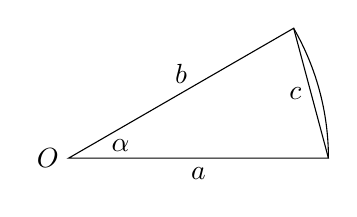
\begin{tikzpicture}[scale=1.1]
  \coordinate  (A) at (3,0);
  \coordinate[label = left:$O$] (O) at (0,0);
  \vertex{O};
  \draw (A) arc(0:30:3) coordinate (B);
  \draw (A) -- node[below] {$a$} (O) -- node[above] {$b$} (B) -- node[left] {$c$} cycle;
  \node[above right,xshift=12pt,yshift=-1pt] at (O) {$\alpha$};
\end{tikzpicture}
\caption{אורכו של מיתר ביחס לקשת בגודל
$\alpha$}\label{fig.length-of-a-chord}
\end{center}
\end{figure}
\begin{eqn}
c^2&=&a^2+b^2-2ab\cos \alpha\\
c&=&\sqrt{2-2\cos \alpha}\\
\lim_{\alpha\rightarrow 0} c&=& \sqrt{2-2\cdot 1}=0\,.
\end{eqn}
מאיור%
~\ref{fig.ratio-of-sine-to-x}
אפשר לראות ש:
\[
\lim_{\alpha \rightarrow 0} \frac{\sin \alpha}{\alpha} = \lim_{\alpha \rightarrow 0} \frac{2\sin \alpha}{2\alpha}\,.
\]
זה היחס בין אורכו של המיתר
$\overline{PQ}$
לאורכו של הקשת
$\widehat{PQ}$.
אבל ראינו שיחס זה שואף ל-%
$1$
כאשר הזווית הנתמכת
$2\alpha$
שואף ל-%
$0$,
ולכן:
\[
\lim_{\alpha \rightarrow 0} \frac{\sin \alpha}{\alpha} = 1\,.
\]
\end{proof}

\begin{figure}[bt]
\begin{center}
\begin{tikzpicture}[scale=1]
  \draw[thin] (-2,0) -- (2,0);
  \draw[thin] (0,-2) -- (0,2);
  \coordinate[label = above left:$A$]  (A) at (-2,0);
  \coordinate[label = above right:$B$] (B) at (2,0);
  \coordinate[label = above left:$O$] (O) at (0,0);
\vertex{O};
  \node[above right,xshift=10pt] at (O) {$\alpha$} 
    node[below right,xshift=10pt] {$\alpha$};
  \coordinate (P) at (40:2);
  \node[above right] at (P) {$P$};
  \coordinate (Q) at (-40:2);
  \node[draw, name path = circle] at (O)
    [circle through = (A)] {};
  \draw (B)
    arc[start angle=0,end angle=40,radius=2cm];
  \draw (B)
    arc[start angle=0,end angle=-40,radius=2cm];
  \node at (2.3,.8) {$\alpha$};
  \node at (2.3,-.8) {$\alpha$};
  \draw[<->] (P) -- node[fill=white,xshift=-6pt] {\sm{\sin \alpha}}
    (P |- O) coordinate (D);
  \draw[<->] (D) -- node[fill=white,xshift=-6pt] {\sm{\sin \alpha}} (Q);
  \node[below right] at (Q) {$Q$};
  \draw (Q) -- node[below] {$1$} (O) -- node[above] {$1$} (P);
\end{tikzpicture}
\caption{היחס בין 
$\sin x$
ל-%
 $x$}\label{fig.ratio-of-sine-to-x}
\end{center}
\end{figure}

%%%%%%%%%%%%%%%%%%%%%%%%%%%%%%%%%%%%%%%%%%%%%%%%%%%%%%%%%%%

%\newpage

\section{משפטי חוצי זווית}\label{a.bisector}
\index{Triangle!angle bisector theorem}

\begin{theorem}\label{thm.angle-bisector}
במשולש
$\triangle ABC$
חוצה הזווית 
$\angle BAC$
חותך את
$\overline{BC}$
ב-%
$D$
(איור%
~\ref{f.angle-bisector}).
אזי:
\[
\frac {\overline{BD}}{\overline{CD}}=\frac {\overline{AB}}{\overline{AC}}\,.
\]
\end{theorem}

\begin{figure}[tb]
\begin{center}
\begin{tikzpicture}[scale=.8]
% Draw base and path two lines at known angles
\draw (0,0) coordinate (b) node[left] {$B$} -- (8,0) coordinate (c) node[right] {$C$};
\path[name path=ba] (b) -- +(50:4.5);
\path[name path=ca] (c) -- +(150:7);
% Get their intersection and draw lines between vertices
\path[name intersections={of=ba and ca,by=a}];
\node[above] at (a) {$A$};
\draw (a) -- (c) -- (b) -- (a);
\path[name path=bc] (b) -- (c);
\path[name path=bisector] (a) -- +(-80:4);
\path[name intersections={of= bc and bisector,by=d}];
\node[below] at (d) {$D$};
\draw (a) -- (d);
\node[below left,xshift=2pt,yshift=-8pt] at (a) {$\alpha$};
\node[below right,xshift=2pt,yshift=-8pt] at (a) {$\alpha$};
\draw (a) -- node[left] {$h$} (a |- b);
\draw (a|-b) rectangle +(7pt,7pt);
\end{tikzpicture}
\end{center}
\caption{משפט חוצה הזווית הפנימית}\label{f.angle-bisector}
\end{figure}
\begin{proof}
נוכיח את המשפט על ידי חישוב השטחים של שני משולשים תוך שימוש בבסיס וגובה (משוואה%
~\ref{eq.area-from-base}),
ובבסיס, זווית וצלע (משוואה%
~\ref{eq.area-from-sine}):
\begin{eqn}
\triangle ABD&=&\frac{1}{2}\overline{BD}h=\frac{1}{2}\overline{AB}\,\overline{AD}\sin \alpha\\
\frac{\overline{BD}}{\overline{AB}}&=&\frac{\overline{AD}\sin \alpha}{h}\\
\triangle ACD&=&\frac{1}{2}\overline{CD}h=\frac{1}{2}\overline{AC}\,\overline{AD}\sin \alpha\\
\frac{\overline{CD}}{\overline{AC}}&=&\frac{\overline{AD}\sin \alpha}{h}\\
\frac{\overline{BD}}{\overline{CD}}&=&\frac{\overline{AB}}{\overline{AC}}\,.
\end{eqn}
\end{proof}

קיים גם משפט חוצה הזווית עבור חוצה הזווית החיצונית:
\index{Triangle!angle bisector theorem}
\begin{theorem}\label{thm.external-angle-bisector}
במשולש
$\triangle ABC$,
$\overline{AE}$,
חוצה הזווית המשלימה לזווית
$\triangle BAC$
(איור%
~\ref{f.angle-bisector-external}),
חותך את ההמשך של
$\overline{BC}$
ב-%
$E$
(איור%
~\ref{f.angle-bisector}).
אזי:
\[
\frac {\overline{BE}}{\overline{CE}}=\frac {\overline{AB}}{\overline{AC}}\,.
\]
\end{theorem}

\begin{figure}[tb]
\begin{center}
\begin{tikzpicture}[scale=1]
% Draw base and path two lines at known angles
\draw (0,0) coordinate (b) node[below] {$B$} -- (6,0) coordinate (c) node[right] {$C$};
\path[name path=ba] (b) -- +(70:2.5);
\draw[name path=ca] (c) -- +(160:7);
% Get their intersection and draw lines between vertices
\path[name intersections={of=ba and ca,by=a}];
\node[above] at (a) {$A$};
\draw (a) -- (c) -- (b) -- (a);
\path[name path=bc] (b) -- (c);
\node[left,xshift=-10pt,yshift=-2pt] at (a) {$\alpha$};
\node[below,xshift=-12pt,yshift=-8pt] at (a) {$\alpha$};
\path[name path=ext-bisector] (a) -- +(-155:4.7);
\draw[name path=ext-bc] (c) -- ($(c)!1.6!(b)$);
\path[name intersections={of=ext-bc and ext-bisector,by=e}];
\draw (a) -- (e) node[below] {$E$};
\coordinate (d) at (a |- b);
\draw (a) -- node[right] {$h$} (d);
\draw (d) rectangle +(6pt,6pt);
\end{tikzpicture}
\end{center}
\caption{משפט חוצה הזווית החיצונית}\label{f.angle-bisector-external}
\end{figure}

%\newpage

\begin{proof} 
$\overline{AC}$
הוא קו ישר ולכן
$\angle EAC=180^\circ-\alpha$:
\begin{eqn}
\triangle ABE&=&\frac{1}{2}\overline{BE}h=\frac{1}{2}\overline{AE}\,\overline{AB}\sin \alpha\\
\triangle ACE&=&\frac{1}{2}\overline{CE}h=\frac{1}{2}\overline{AE}\,\overline{AC}\sin (180^\circ-\alpha)=\frac{1}{2}\overline{AE}\,\overline{AC}\sin \alpha\\
\frac{\overline{BE}}{\overline{AB}}&=&\frac{\overline{AE}\sin \alpha}{h}=\frac{\overline{CE}}{\overline{AC}}\\
\frac{\overline{BE}}{\overline{CE}}&=&\frac{\overline{AB}}{\overline{AC}}\,.
\end{eqn}
\end{proof}

%%%%%%%%%%%%%%%%%%%%%%%%%%%%%%%%%%%%%%%%%%%%%%%%%%%%%%%%%%%

\newpage

\section{משפט
\L{\normalsize Ptolemy}}\label{a.ptolemy}
\index{Ptolemy's theorem}

%%%%%%%%%%%%%%%%%%%%%%%%%%%%%%%%%%%%%%%%%%%%%%%%%%%%%%%%%%%

\subsection{מעגל החסום על ידי טרפז}\label{s.circumscribed}

לפי שנוכיח את משפט
\L{Ptolemy}
נוכיח משפטים על מרובעים וטרפזים.

\begin{theorem}\label{thm.quad-circum}
ניתן לחסום מרובע במעגל אם ורק אם הזוויות הנגדיות משלימות (הסכום שווה ל-%
$180^\circ$).
\end{theorem}\index{Circumscribed circle}

ספרי לימוד בגיאומטריה מביאים הוכחה פשוטה של הכיוון "רק אם", אבל קשה למצוא הוכחה של הכיוון "אם", לכן אביא פה את שתי ההוכחות.

\begin{proof}
(רק אם)
זווית היקפית במעגל שווה למחצית הקשת שתומך בו כך ש-%
$\angle DAB$
שווה לחצי הקשת 
$\widehat{DCB}$
ו-%
$\angle DCB$
שווה לחצי הקשת
$\widehat{DAB}$ 
(איור~%
\ref{f.trap-1}).
שתי הקשתות ביחד מקיפים את כל היקף המעגל ולכן סכומן 
$360^\circ$. 
מכאן ש-%
$\angle DAB + \angle DCB = 180^\circ$
ו-%
$\angle ADC + \angle ABC = 180^\circ$.

\end{proof}

\begin{figure}[tb]
\centering
\selectlanguage{hebrew}
\subcaptionbox{%
מרובע חסום על ידי מעגל
\label{f.trap-1}}
[.45\textwidth]
{
\centering
\begin{tikzpicture}[scale=.55]
\coordinate (origin) at (0,0);
\coordinate (A) at (1,3);
\node[draw,circle through=(A),name path=circle] at (origin) {};
\node[above right] at (A) {$A$};
\path[name path=b] (A) -- (-50:4.5cm);
\path[name path=c] (A) -- (-120:4.5cm);
\path[name path=d] (A) -- (150:4.5cm);
\path [name intersections={of=circle and b,by={b1,B}}];
\node[right] at (B) {$B$};
\path [name intersections={of=circle and c,by={c1,C}}];
\node[below left] at (C) {$C$};
\path [name intersections={of=circle and d,by={d1,D}}];
\node[above left] at (D) {$D$};
\draw (A) -- (B) -- (C) -- (D) -- cycle;
\end{tikzpicture}
}
\hspace{3em}
\subcaptionbox{%
הקודקוד
$C$
חייב להיות על היקף המעגל
\label{f.trap-2}}
[.45\textwidth]
{
\centering
\begin{tikzpicture}[scale=.55]
\coordinate (origin) at (0,0);
\coordinate (A) at (1,3);
\node[draw,circle through=(A),name path=circle] at (origin) {};
\node[above right] at (A) {$A$};
\path[name path=b] (A) -- (-50:4cm);
\path[name path=c] (A) -- (-120:4cm);
\path[name path=d] (A) -- (150:4cm);
\path [name intersections={of=circle and b,by={b1,B}}];
\node[right] at (B) {$B$};
\path [name intersections={of=circle and c,by={c1,C}}];
\node[below left] at (C) {$C$};
\path [name intersections={of=circle and d,by={d2,D}}];
\node[above left] at (D) {$D$};
\coordinate (Cp) at ($(C)!.2!(D)$);
\draw (A) -- (B) -- (Cp) -- (D) -- cycle;
\node[left,xshift=1pt,yshift=2pt] at (Cp) {$C'$};
\draw (D) -- (B) -- (C) -- (Cp);
\end{tikzpicture}
}
\end{figure}

\begin{proof} 
(אם)
ניתן לחסום כל משולש על ידי מעגל. נחסום את 
$\triangle DAB$
במעגל ונניח שיש נקודה 
$C'$
כך ש-%
$\angle DAB + \angle DC'B = 180^\circ$, 
אבל
$C'$
\textbf{לא נמצאת}
על היקף המעגל. ללא הגבלת הכלליות נניח ש-%
$C'$
נמצאת בתוך המעגל 
(איור~%
\ref{f.trap-2}).

בנה קרן שמאריכה את 
$\overline{DC'}$
ותהי 
$C$
נקודת החיתוך שלה עם המעגל.
$\overline{ABCD}$
חסום על ידי מעגל ולכן:
\index{Circumscribed circle}
\begin{eqn}
\angle DAB + \angle DCB &=&  180^\circ = \angle DAB + \angle DC'B\\
\angle DCB &=& \angle DC'B\,,
\end{eqn}
תוצאה שאינה אפשרית אם 
$C$
נמצאת על היקף המעגל ו-%
$C'$
נמצאת בתוך המעגל.
\end{proof}

\newpage

\begin{theorem}\label{thm.isoceles-trapezoid}
הזוויות הנגדיות של טרפז שווה-שוקיים משלימות.
\end{theorem}\index{Trapezoid, isoceles}\index{Circumscribed circle!trapezoid@around a trapezoid}
\begin{proof}
נבנה קו 
$\overline{AB'}$
מקביל ל-%
$\overline{CD}$
(איור%
~\ref{f.trap-3}).
$\overline{AB'CD}$
מקבילית ו-%
$\triangle ABB'$
משולש שווה-שוקיים, ולכן
$\angle C= \angle ABB' = \angle AB'B = \angle B$.
באופן דומה
$\angle A = \angle D$.
סכום הזוויות הפנימיות של מרובע הוא 
$360^\circ$
ולכן:
\begin{eqn}
\angle A + \angle B + \angle C + \angle D &=& 360^\circ\\
2\angle A + 2 \angle C &=& 360^\circ\\
\angle A +  \angle C &=& 180^\circ\,,
\end{eqn}
ובאופן דומה
$\angle B +  \angle D = 180^\circ$.
\end{proof}

\begin{theorem}
ניתן לחסום טרפז שווה-שוקיים על ידי מעגל.
\end{theorem}
ההוכחה מיידית מהמשפטים%
\ref{thm.quad-circum}, ~\ref{thm.isoceles-trapezoid}.

\begin{figure}[tb]
\begin{center}
\begin{tikzpicture}[scale=.65]
\clip (-4.5,-2) rectangle (4.5,2.8);
\coordinate (origin) at (0,0);
\coordinate (A) at (2.5,1.8);
\node[circle through=(A),name path=circle] at (origin) {};
\node[above right] at (A) {$A$};
\path[name path=b] (A) -- ++(-80:4cm);
\path[name path=d] (A) -- ++(180:6cm);
\path [name intersections={of=circle and b,by={b1,B}}];
\node[below right] at (B) {$B$};
\path [name intersections={of=circle and d,by={d1,D}}];
\node[above left] at (D) {$D$};
\path[name path=c] (D) -- ++(-100:4cm);
\path [name intersections={of=circle and c,by={c1,C}}];
\node[below left] at (C) {$C$};
\draw (A) -- node[right] {$x$} (B);
\draw[name path=bc] (B) -- node[below] {$y$} (C);
\draw (C) -- node[left] {$x$} (D) -- node[above] {$y$} (A);
\path[name path=para] (A) -- ++(-100:4cm);
\path [name intersections={of=para and bc,by={Bp}}];
\node[below left] at (Bp) {$B'$};
\draw (A) -- node[left,xshift=-2pt] {$x$} (Bp);
\end{tikzpicture}
\end{center}
\caption{טרפז שווה-שוקיים}\label{f.trap-3}
\end{figure}

%%%%%%%%%%%%%%%%%%%%%%%%%%%%%%%%%%%%%%%%%%%%%%%%%%%%%%%%%%%
\subsection{הוכחת המשפט של \L{Ptolemy}}

\begin{theorem}[\L{Ptolemy}]
נתון מרובע חסום על ידי מעגל, הנוסחה שלהלן מתאר את הקשר בין אורכי האלכסונים ואורכי הצלעות
(איור%
~\ref{f.trig-ptolemy}).\label{thm.ptolemy}\index{Circumscribed circle}
\[
ef = ac + bd\,.
\]
\end{theorem}

\begin{figure}[tb]
\begin{center}
\begin{tikzpicture}[scale=.5]
\coordinate (origin) at (0,0);
\coordinate (A) at (1,3);
\node[draw,circle through=(A),name path=circle] at (origin) {};
\node[above right] at (A) {$A$};
\path[name path=b] (A) -- (-50:4cm);
\path[name path=c] (A) -- (-120:4cm);
\path[name path=d] (A) -- (150:4cm);
\path [name intersections={of=circle and b,by={b1,B}}];
\node[right] at (B) {$B$};
\path [name intersections={of=circle and c,by={C,c2}}];
\node[below left] at (C) {$C$};
\path [name intersections={of=circle and d,by={D,d2}}];
\node[above left] at (D) {$D$};
\draw (A) -- node[right] {$a$} (B) -- node[below,yshift=-10pt] {$b$} (C) -- node[left] {$c$} (D) -- node[above,xshift=2pt,yshift=8pt] {$d$}  cycle;
\draw (A) -- node[right,near start] {$e$} (C);
\draw (B) -- node[left,near end,yshift=-6pt] {$f$} (D);
\end{tikzpicture}
\end{center}
\caption{משפט \L{Ptolemy}}\label{f.trig-ptolemy}
\end{figure}                       

\begin{proof}
לפי חוק הקוסינוס עבור ארבעת המשולשים
\index{Law of cosines}
$\triangle ABC$, $\triangle ADC$, $\triangle DAB$, $\triangle DCB$:
\begin{eqn}
e^2 &=& a^2 + b^2 - 2ab \cos \angle B\\
e^2 &=& c^2 + d^2 - 2cd \cos \angle D\\
f^2 &=& a^2 + d^2 - 2ad \cos \angle A\\
f^2 &=& b^2 + c^2 - 2bc \cos \angle C\,.
\end{eqn}
$\angle C = 180^\circ - \angle A$
ו=%
$\angle D = 180^\circ - \angle B$
כי הן זוויות נגדיות של מרובע חסום על ידי מעגל, ולכן
$\cos \angle D = - \cos \angle B$
ו-%
$\cos \angle C = -\cos \angle A$.
נצמצם את הקוסינוס כדי לקבל:
\begin{eqn}
e^2(cd+ab)&=&abc^2+abd^2+a^2cd+b^2cd\\
e^2 &=& \frac{(ac+bd)(ad+bc)}{(ab+cd)}\\
f^2 &=& \frac{(ab+cd)(ac+bd)}{(ad+bc)}\,.
\end{eqn}
הכפל את שתי המשוואות ופשט כדי לקבל את משפטו של
\L{Ptolemy}:
\begin{eqn}
e^2\cdot f^2 &=& (ac+bd)^2\\
ef &=& (ac+bd)\,.
\end{eqn}
\end{proof}

%%%%%%%%%%%%%%%%%%%%%%%%%%%%%%%%%%%%%%%%%%%%%%%%%%%%%%%%%%%

\section{המשפט של
\L{\normalsize Ceva}}\label{a.ceva}

\index{Ceva's theorem}\label{thm.ceva}
\begin{theorem}[Ceva]
נתון קטעי קו מהקודקודים של משלוש לצלעות הנגדיות שנחתכים בנקודה, אורכי הקטעים מקיימים את הנוסחה (איור%
~\ref{f.ceva1}):
\[
\frac{\overline{AM}}{\overline{MB}}\cdot\frac{\overline{BQ}}{\overline{QS}}\cdot\frac{\overline{SP}}{\overline{PA}} = 1\,.
\]
\end{theorem}

\begin{figure}[tb]
\begin{center}
\begin{tikzpicture}
\path[name path=pq] (-4,0) -- (4,0);
\draw (-2,-2) node[below left] {$A$} coordinate (A) -- (2,-2) node[below right] {$B$} coordinate (B);
\draw[name path=as] (A) -- ++(50:4cm) node[above] {$S$} coordinate (S);
\draw[name path=sb] (S) -- (B);
\path [name intersections={of=pq and as,by={P}}];
\path [name intersections={of=pq and sb,by={Q}}];
\node[above left] at (P) {$P$};
\node[above right] at (Q) {$Q$};
\draw[name path=pb] (P) -- (B);
\draw[name path=qa] (Q) -- (A);
\path [name intersections={of=pb and qa,by={O}}];
\node[right,xshift=2pt] at (O) {$O$};
\coordinate (M) at (0,-2);
\node[below right] at (M) {$M$};
\draw (S) -- (M);
\end{tikzpicture}
\end{center}
\caption{משפט \L{Ceva}}\label{f.ceva1}
\end{figure}

\begin{proof}
אם הגבהים של שני משולשים שווים, אזי היחסים בין השטחים שווים ליחסים בין לבסיסים. בשתי התרשימים באיור%
~\ref{f.ceva2}
הגבהים של המשולשים האפורים שווים ולכן:
\[
\frac{\triangle BQO}{\triangle SQO} = \frac{\overline{BQ}}{\overline{QS}}\;,\quad\quad \frac{\triangle BQA}{\triangle SQA} = \frac{\overline{BQ}}{\overline{QS}}\;.
\]
נחסיר את השטחים האפרים במשולשים ונקבל את היחס בין המשלושים האפורים באיור%
~\ref{f.ceva3}:
\[
\frac{\triangle BOA}{\triangle SOA}=\frac{\triangle BQA - \triangle BQO}{\triangle SQA-\triangle SQO} = \frac{\overline{BQ}}{\overline{QS}}\,.
\]

\begin{figure}[tb]
\begin{center}
\begin{tikzpicture}
\clip (-2.2,-2.4) rectangle +(10.4,4);
\path[name path=pq] (-4,0) -- (4,0);
\draw (-2,-2) node[below] {$A$} coordinate (A) -- (2,-2) node[below] {$B$} coordinate (B);
\coordinate (M) at (0,-2);
\draw[name path=as] (A) -- ++(50:4cm) node[above] {$S$} coordinate (S);
\draw[name path=sb] (S) -- (B);
\path [name intersections={of=pq and as,by={P}}];
\path [name intersections={of=pq and sb,by={Q}}];
\path[name path=pb] (P) -- (B);
\path[name path=qa] (Q) -- (A);
\path [name intersections={of=pb and qa,by={O}}];
\draw[fill=gray!40] (B) -- (O) -- (Q);
\draw[fill=gray!70] (S) -- (O) -- (Q);
\draw (B) -- (O) -- (A);
\draw (S) -- (O) -- (A);
\draw (A) -- (B) -- (S) -- cycle;
\draw (S) -- (O);
\draw (B) -- (O);
\node[above right] at (Q) {$Q$};
\node[above left] at (O) {$O$};
\path[name path=al1] (O) -- ($(Q)!(O)!(B)$);
\path [name intersections={of=al1 and sb,by={A1}}];
\draw (O) -- (A1);
\draw[rotate=-156] (A1) rectangle +(7pt,7pt);
\begin{scope}[xshift=6cm]
\path[name path=pq] (-4,0) -- (4,0);
\draw (-2,-2) node[below] {$A$} coordinate (A) -- (2,-2) node[below] {$B$} coordinate (B);
\coordinate (M) at (0,-2);
\draw[name path=as] (A) -- ++(50:4cm) node[above] {$S$} coordinate (S);
\draw[name path=sb] (S) -- (B);
\path [name intersections={of=pq and as,by={P}}];
\path [name intersections={of=pq and sb,by={Q}}];
\draw[name path=pb] (P) -- (B);
\draw[name path=qa] (Q) -- (A);
\path [name intersections={of=pb and qa,by={O}}];
\draw (B) -- (O) -- (Q);
\draw (A) -- (Q) -- (B);
\draw[fill=gray!40] (B) -- (Q) -- (A);
\draw[fill=gray!70] (S) -- (Q) -- (A);
\draw (A) -- (B) -- (S) -- cycle;
\draw (S) -- (O);
\draw (B) -- (O);
\node[above right] at (Q) {$Q$};
\node[above left] at (O) {$O$};
\path[name path=al2] (A) -- ($(Q)!(A)!(B)$);
\path [name intersections={of=al2 and sb,by={A2}}];
\draw (A) -- (A2);
\draw[rotate=-156] (A2) rectangle +(7pt,7pt);
\end{scope}
\end{tikzpicture}
\end{center}
\caption{משולשים במשפט \L{Ceva}}\label{f.ceva2}
\end{figure}

\begin{figure}[tb]
\begin{center}
\begin{tikzpicture}
\path[name path=pq] (-4,0) -- (4,0);
\draw (-2,-2) node[below left] {$A$} coordinate (A) -- (2,-2) node[below right] {$B$} coordinate (B);
\coordinate (M) at (0,-2);
\draw[name path=as] (A) -- ++(50:4cm) node[above] {$S$} coordinate (S);
\draw[name path=sb] (S) -- (B);
\path [name intersections={of=pq and as,by={P}}];
\path [name intersections={of=pq and sb,by={Q}}];
\path[name path=pb] (P) -- (B);
\draw[thick,name path=qa] (Q) -- (A);
\path [name intersections={of=pb and qa,by={O}}];
\draw[fill=gray!50] (B) -- (O) -- (A);
\draw[fill=gray!70] (S) -- (O) -- (A);
\draw (B) -- (O) -- (A);
\draw (S) -- (O) -- (A);
\draw (A) -- (B) -- (S) -- cycle;
\draw (S) -- (O);
\draw (B) -- (O);
\node[above right] at (Q) {$Q$};
\node[right,xshift=2pt] at (O) {$O$};
\end{tikzpicture}
\end{center}
\caption{החסרת שטחים במשפט \L{Ceva}}\label{f.ceva3}
\end{figure}

חישוב זה עלול להיראות מעט מוזר אז נסביר אותו בסימון פשוט יותר:
\begin{eqn}
 \frac{c}{d} &=&\frac{a}{b}\\
 \frac{e}{f} &=&\frac{a}{b}\\
c-e &=& \frac{ad}{b} - \frac{af}{b}=\frac{a}{b}(d-f)\\
\frac{c-e}{d-f} &=& \frac{a}{b}\,.
\end{eqn}

%\newpage

באופן דומה ניתן להוכיח:
\begin{eqn}
\frac{\overline{AM}}{\overline{MB}} &=& \frac{\triangle AOS}{\triangle BOS}\\
\frac{\overline{SP}}{\overline{PA}} &=&\frac{\triangle SOB}{\triangle AOB}\;,
\end{eqn}
ולכן:
\[
\frac{\overline{AM}}{\overline{MB}}\frac{\overline{BQ}}{\overline{QS}}\frac{\overline{SP}}{\overline{PA}} = \frac{\triangle AOS}{\triangle BOS}\frac{\triangle BOA}{\triangle SOA}\frac{\triangle SOB}{\triangle AOB}=1\,,
\]
כי הסדר של הקודקודים במשולש לא משנה.
\end{proof}

\begin{figure}[tb]
\begin{center}
\begin{tikzpicture}[scale=.8]
\clip (-.8,-.4) rectangle +(11.2,6.5);
\coordinate (D) at (0,0) node[left] {$D$};
\draw (D) -- ++(60:6) coordinate (C) node[left] {$C$};
\coordinate (A) at (60:3);
\node[left] at (A) {$A$};
\draw (A) -- ++(3,0) coordinate (B) -- (C);
\node[below right] at (B) {$B$};
\path[name path=DQ] (D) -- ($(D)!1.7!(B)$);
\path[name path=AP] (A) -- ($(A)!3!(B)$);
% 3*(1+\sqrt[3]{2}) = 6.78
\path[name path=CP] (C) circle (6.78cm);
\path[name intersections={of=CP and AP,by={P}}];
\draw[name path=CP] (C) -- (P);
\path[name intersections={of=CP and DQ,by={Q}}];
\node[above] at (Q) {$Q$};
\node[right] at (P) {$P$};
\draw (D) -- (Q);
\draw (B) -- (P);
\path[dashed,name path=CK] (C) -- ($(C)+(6.5,0)$);
\path[name path=DK] (D) -- ($(D)!2!(Q)$);
\path[name intersections={of=DK and CK,by={K}}];
\draw[dashed] (Q) -- (K) node[right] {$K$} -- (C);
\draw[very thick] (Q) -- (D);
\draw[dashed] (C) -- (K) -- (Q);
\draw (B) -- (P) -- (C);
\end{tikzpicture}
\end{center}
\caption{המשפט של \L{Menelaus}}\label{f.menelaus}
\end{figure}

%%%%%%%%%%%%%%%%%%%%%%%%%%%%%%%%%%%%%%%%%%%%%%%%%%%%%%%%%

\section{המשפט של
\L{\normalsize Menelaus}}\label{a.menelaus}

\begin{theorem}[\L{Menelaus}]\label{thm.menelaus}\index{Menelaus's theorem}
יהי 
$\triangle ABC$
משולש ויהי 
$\overline{DBQ}$
\textbf{קו חותך}
\L{(transveral)}
החותך את שלושת הצלעות של המשולש או את ההארכות שלהם
(איור.~\ref{f.menelaus}).
אזי:%
\footnote{%
כתלות המבנה המשולשים והקו החותך, המכלפה יכולה להיות
$+1$
או
$-1$.}
\begin{equation}
\displaystyle\frac{\overline{AB}}{\overline{BP}}\cdot
\displaystyle\frac{\overline{PQ}}{\overline{QC}}\cdot
\displaystyle\frac{\overline{CD}}{\overline{AD}}=1\,.\label{eq.menelaus}
\end{equation}
\end{theorem}

\begin{proof}
נבנה קו דרך 
$C$
המקביל ל-%
$\overline{AB}$
ונאריך את
$\overline{DQ}$
עד שהוא חותך את הקו המקביל ב-%
$K$.
מ-%
$\triangle ADB \sim \triangle CDK$
נובע:
\[
\displaystyle\frac{\overline{CD}}{\overline{AD}}=\displaystyle\frac{\overline{CK}}{\overline{AB}}\,.
\]
מ-%
$\triangle  BQP\sim \triangle KQC$
נובע:
\[
\displaystyle\frac{\overline{QC}}{\overline{PQ}}=\displaystyle\frac{\overline{CK}}{\overline{BP}}\,.
\]
נצמצם את 
$\overline{CK}$
ונקבל
$\overline{AB}\cdot\overline{CD}\cdot\overline{PQ}=\overline{QC}\cdot\overline{BP}\cdot\overline{AD}$ 
שניתן לסדר מחדש כדי לקבל את המשוואה%
~\ref{eq.menelaus}.
\end{proof}

%%%%%%%%%%%%%%%%%%%%%%%%%%%%%%%%%%%%%%%%%%%%%%%%%%%%%%%%%%%

\subsection*{מקורות}

פרק זה מבוסס בעיקר על
\cite{gelfand}.
ניתן להוכיח את משפט
\L{Ceva}
ומשפט
\L{Menelaus}
אחד המשני
\cite{silvester}.
